\documentclass[final]{beamer}

% ====================
% Packages
% ====================

\usepackage[T1]{fontenc}
\usepackage{lmodern}
\usepackage[size=a1,scale=1.0]{beamerposter}
\usetheme{gemini}
\usecolortheme{UNR}
\usepackage{graphicx}
\usepackage{booktabs}
\usepackage{svg}
\usepackage{pgfplots}
\usepackage{lipsum}

% ====================
% Lengths
% ====================

% If you have N columns, choose \sepwidth and \colwidth such that
% (N+1)*\sepwidth + N*\colwidth = \paperwidth
\newlength{\sepwidth}
\newlength{\colwidth}
\setlength{\sepwidth}{0.025\paperwidth}
\setlength{\colwidth}{0.3\paperwidth}

\newcommand{\separatorcolumn}{\begin{column}{\sepwidth}\end{column}}

% ====================
% Title
% ====================

\title{DeadDrop}

\author{Jann Arellano, Brian Buslon\\Keaton Clark, Lloyd Gonzales}

\institute[shortinst]{CSE Department, UNR \and \textbf{Advisor:} Shamik Sengupta. Professor. University of Nevada, Reno \and \textbf{Instructors:} David Feil-Seifer, Devrin Lee, Sara Davis}

% remove this section if poster is for inhouse project
\addtobeamertemplate{headline}{} 
{
    \begin{tikzpicture}[remember picture,overlay]
    % tweak these sizes according to the logo of the company:
    % xshift, yshift, height
    \node [anchor=north west, inner sep=3cm] at ([xshift=-1.5cm,yshift=1.6cm]current page.north west)     {
\includegraphics[height=5cm]{images/unr.png}}; 
    \end{tikzpicture} 
}

% ====================
% Body
% ====================

\begin{document}


\begin{frame}[t]
\begin{columns}[t]
\separatorcolumn

\begin{column}{\colwidth}

  \begin{alertblock}{Abstract}
    \textbf{Reduce the size of this}
    \it{
      DeadDrop is a command and control (C2) framework used in post-exploitation activities and penetration testing to create malware payloads, manage compromised devices and generate operational reports.
      DeadDrop's primary purpose is to aid legitimate security professionals (the "red team") in an activity known as penetration testing, which assesses a company's ability to defend against attacks and protect its data.
      Penetration tests often are coordinated using C2 frameworks, which significantly simplifies managing infected devices while ensuring accountability for actions taken by the red team.
      Using a C2 framework in testing greatly benefits security engineers (the "blue team"), as they can identify opportunities through the reporting and logging functionality provided by the C2 framework.
      However, unlike existing frameworks, DeadDrop focuses on leveraging features in legitimate websites such as YouTube and Wikipedia to communicate with devices and exfiltrate data, masking its activity within the noise of popular websites.
      Messages (dead drops) can be placed on external services by one device, which can be retrieved by the other device by accessing the external service.
      By abusing the "trust" behind large, well-known websites, DeadDrop provides security engineers with new insight into identifying covert attacker techniques and security weaknesses.
    }
  \end{alertblock}

  \begin{block}{More Description}

    Et rutrum ex euismod vel. Pellentesque ultricies, velit in fermentum
    vestibulum, lectus nisi pretium nibh, sit amet aliquam lectus augue vel
    velit. Suspendisse rhoncus massa porttitor augue feugiat molestie. Sed
    molestie ut orci nec malesuada. Sed ultricies feugiat est fringilla
    posuere.

    \begin{figure}
      \centering
      \begin{tikzpicture}
        \begin{axis}[
            scale only axis,
            no markers,
            domain=0:2*pi,
            samples=100,
            axis lines=center,
            axis line style={-},
            ticks=none]
          \addplot[red] {sin(deg(x))};
          \addplot[blue] {cos(deg(x))};
        \end{axis}
      \end{tikzpicture}
      \caption{Another figure caption.}
    \end{figure}

  \end{block}


\end{column}

\separatorcolumn

\begin{column}{\colwidth}

  \begin{block}{Project overview}

    Vivamus congue volutpat elit non semper. Praesent molestie nec erat ac
    interdum. In quis suscipit erat. \textbf{Phasellus mauris felis, molestie
    ac pharetra quis}, tempus nec ante. Donec finibus ante vel purus mollis
    fermentum. Sed felis mi, pharetra eget nibh a, feugiat eleifend dolor. Nam
    mollis condimentum purus quis sodales. Nullam eu felis eu nulla eleifend
    bibendum nec eu lorem. Vivamus felis velit, volutpat ut facilisis ac,
    commodo in metus.

    \begin{enumerate}
      \item \textbf{Morbi mauris purus}, egestas at vehicula et, convallis
        accumsan orci. Orci varius natoque penatibus et magnis dis parturient
        montes, nascetur ridiculus mus.
      \item \textbf{Cras vehicula blandit urna ut maximus}. Aliquam blandit nec
        massa ac sollicitudin. Curabitur cursus, metus nec imperdiet bibendum,
        velit lectus faucibus dolor, quis gravida metus mauris gravida turpis.
      \item \textbf{Vestibulum et massa diam}. Phasellus fermentum augue non
        nulla accumsan, non rhoncus lectus condimentum.
    \end{enumerate}

  \end{block}

  \begin{block}{Architecture}

    Nam vulputate nunc felis, non condimentum lacus porta ultrices. Nullam sed
    sagittis metus. Etiam consectetur gravida urna quis suscipit.

    Some block contents, followed by a diagram, followed by a dummy paragraph.

    \begin{figure}
      \centering
      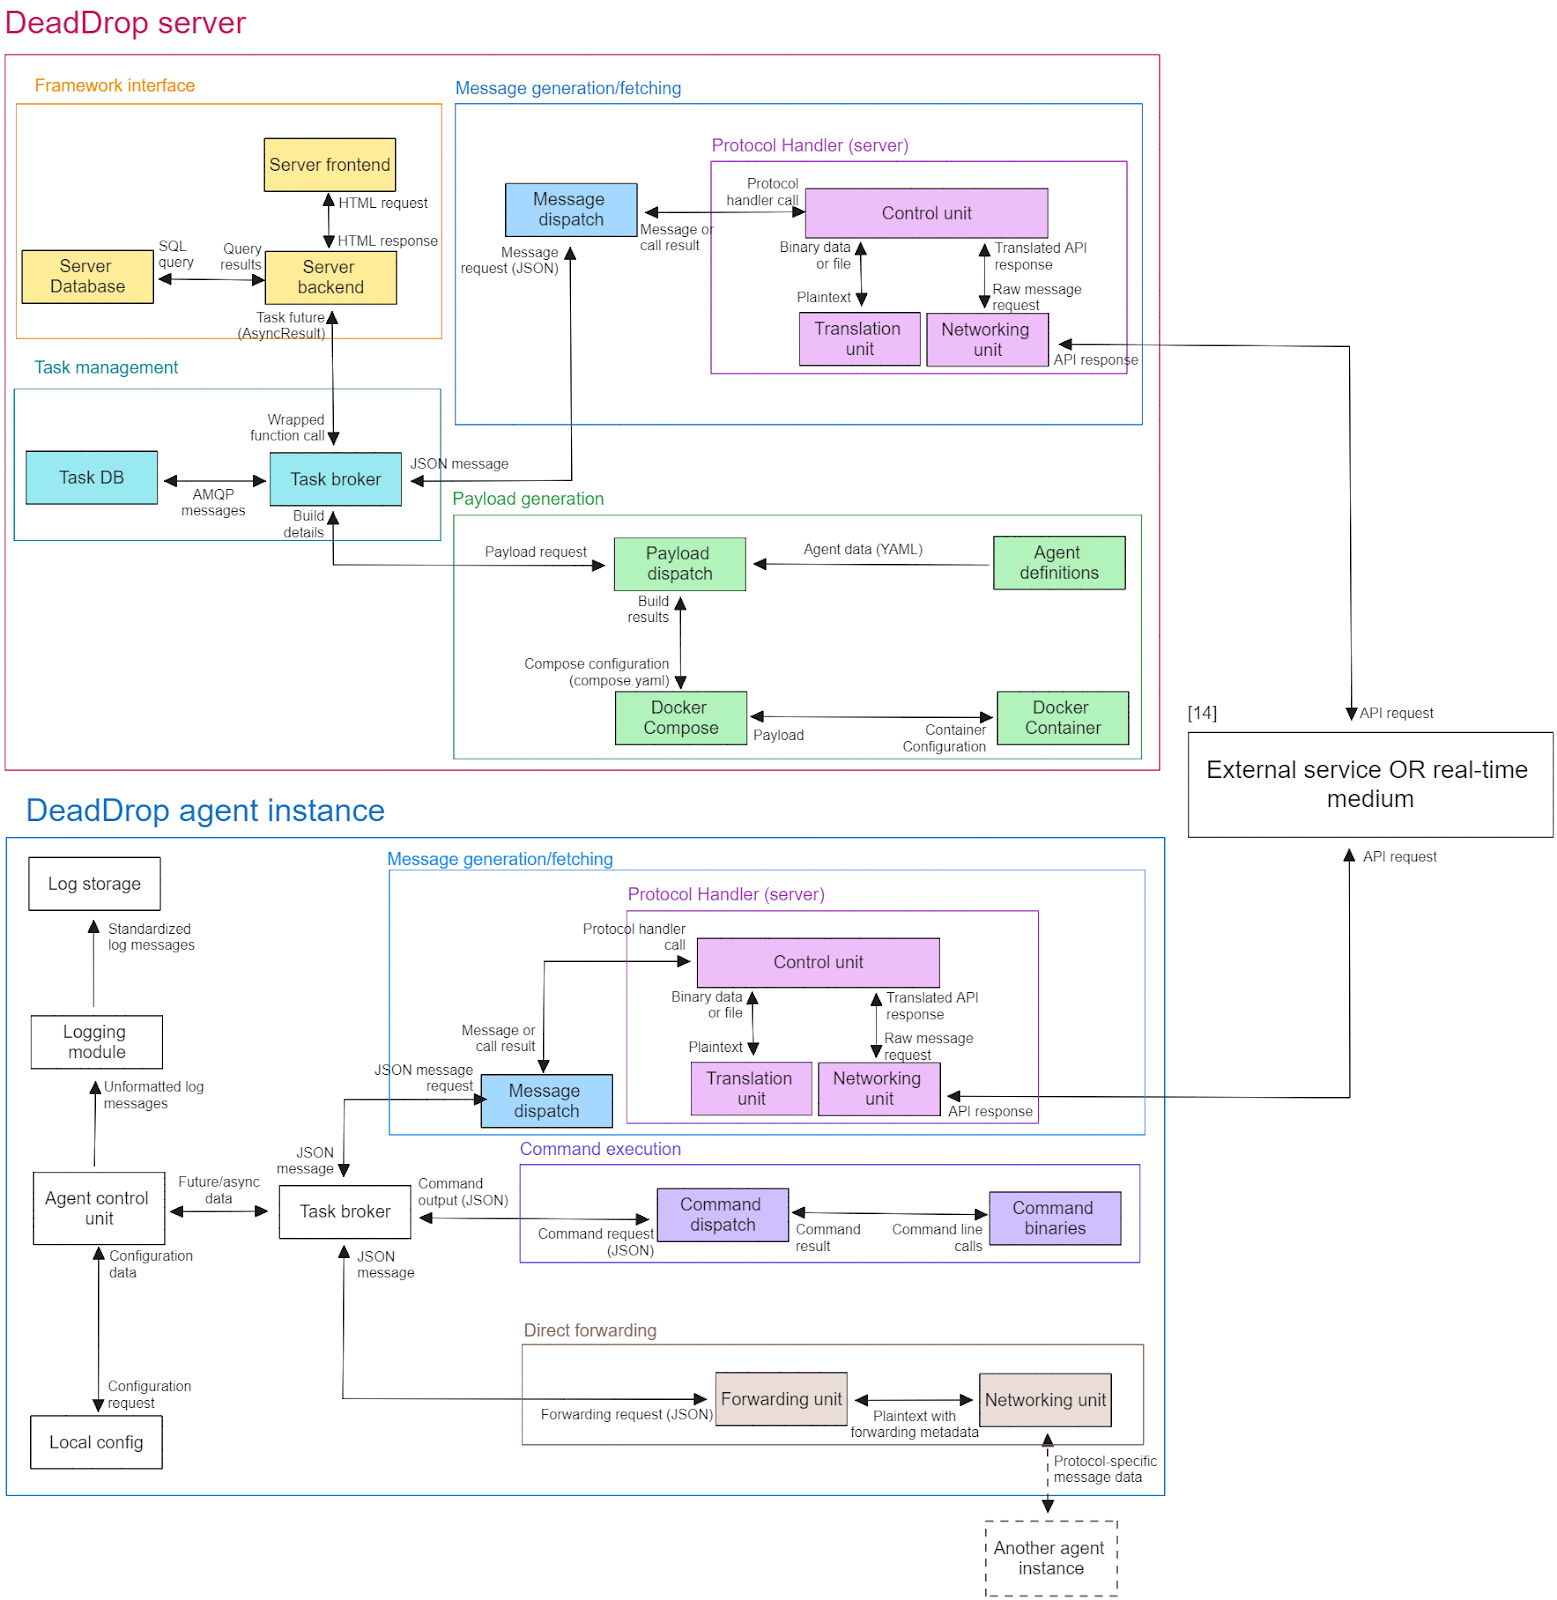
\includegraphics[width=\textwidth]{images/architecture.png}
      \caption{Get svg}
    \end{figure}

  \end{block}

\end{column}

\separatorcolumn

\begin{column}{\colwidth}

  \begin{block}{Future Work}

    \heading{Near Future}

    \lipsum[1]

    \heading{Far Future}

    \lipsum[1]

  \end{block}

  \begin{block}{Conclusion}

    \lipsum[1]

  \end{block}

  \begin{block}{References}
    \nocite{*}
    \footnotesize{\bibliographystyle{plain}\bibliography{poster}}
  \end{block}
  
  \begin{block}{}
    
    \it{This project was developed in Spring 2023 as part of the course CS 426 Senior Projects in Computer Science}

  \end{block}

\end{column}

\separatorcolumn
\end{columns}
\end{frame}

\end{document}
